\documentclass[11pt,compress,t,notes=noshow, aspectratio=169, xcolor=table]{beamer}

\usepackage{../../style/lmu-lecture}
% Defines macros and environments
 
%\title{iML: Post-hoc Methods for Neural Networks}
%\subtitle{Simple gradients, Integrated gradients}
%\newcommand{\tikzmark}[1]{\tikz[baseline,remember picture] \coordinate (#1) {};}

\title{Interpretable Machine Learning}
\date{}
\begin{document}
	%\maketitle
	\graphicspath{ {./figure/} }

\newcommand{\titlefigure}{figure/bild15}
\newcommand{\learninggoals}{
\item Basics of sensitivity analysis
\item Saliency maps for images and language
\item integrated gradients}

\lecturechapter{Simple Gradients \& Integrated Gradients}
\lecture{Interpretable Machine Learning}


\begin{frame}{Sensitivity Analysis}
    \begin{itemize}
        \item Neural Networks are differentiable machines
        \begin{itemize}
            \item The output can be written as a function of the parameters and input
            \item One can differentiate the output function w.r.t parameters
            \item The underlying idea is used for training Neural Nets using gradient descent
            \begin{equation*}
                f(x;\theta)\hspace{4cm}  \frac{\partial f(x;\theta)}{\partial\theta}
            \end{equation*}
        \end{itemize}
        \item Sensitivity Analysis: How sensitive is the output $f()$ w.r.t to a small change in the
input?
    \end{itemize}
    \pause
    \bigskip
     \begin{equation*}
                 \frac{\partial f(x;\theta)}{\partial x}
            \end{equation*}
\end{frame}
	
\begin{frame}{Sensitivity Analysis}
    \begin{itemize}
        \item How sensitive is the output $f() $w.r.t to a small change in the input ?
        \begin{itemize}
            \item If a small change in the input feature causes a large change in output, then that
feature is responsible for the prediction
\item Back-propagation into the input: instead of computing \quad $\frac{\partial f(x;\theta)}{\partial\theta}$
        \end{itemize}
    \end{itemize}
\begin{figure}
    \centering
    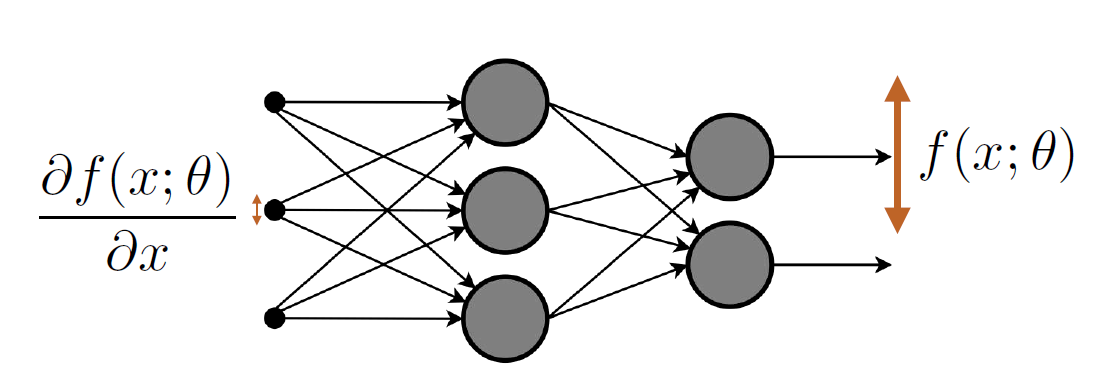
\includegraphics[scale=.45]{bild14}
\end{figure}    
\end{frame}

\begin{frame}{Saliency Maps}
\begin{itemize}
    \item Visualize the gradients over each feature
    \begin{itemize}
        \item as a heat map or Saliency Maps %color?
        \item Saliency maps are feature attribution methods that are based on gradients
    \end{itemize}
    \bigskip
    \begin{figure}
        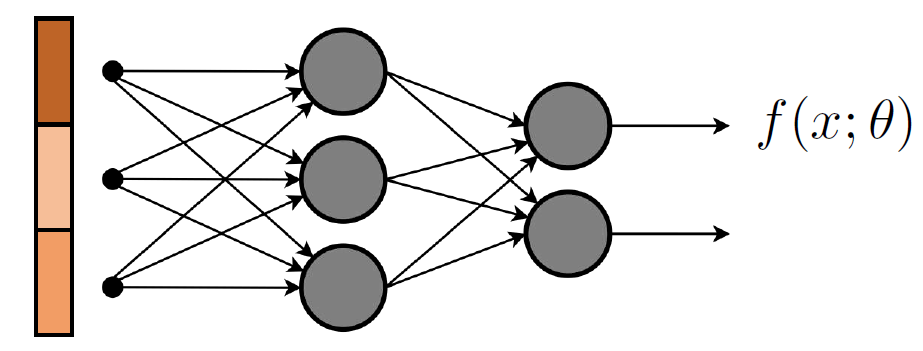
\includegraphics[scale=.5]{bild15}
    \end{figure}
\end{itemize}

\end{frame}

\begin{frame}{Saliency Maps for Images}
    \begin{itemize}
        \item Images have multiple channels where each channel is a 2-D matrix
    \end{itemize}
    \begin{equation*}
        M_{ij} = \underset{c}{\text{max}}\left|\nabla_xS_c(X) \right|_{(i,j,c)}
    \end{equation*}
    \begin{figure}
        \centering
        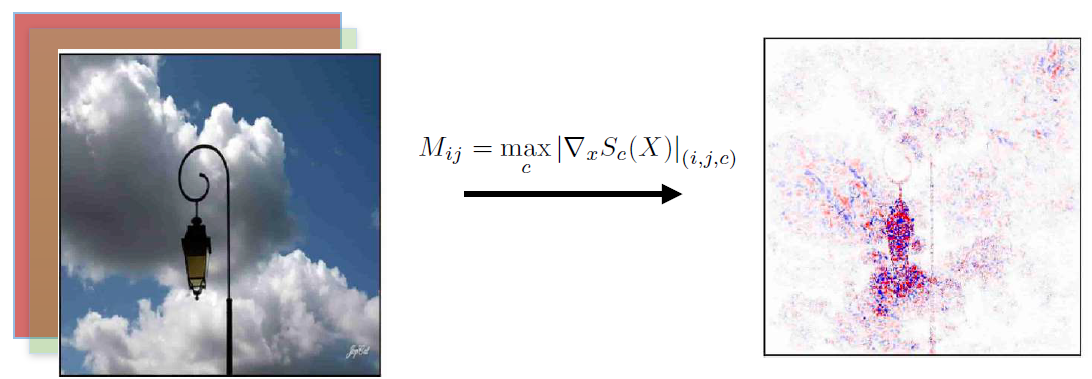
\includegraphics[scale=.45]{bild16n}
    \end{figure}
\end{frame}

\begin{frame}{Saliency Maps for Language}
    \begin{itemize}
        \item Words are associated with an embedding
        \item Computing gradients back to the inputs is different in comparison to images
    \end{itemize}
    \begin{figure}
        \centering
        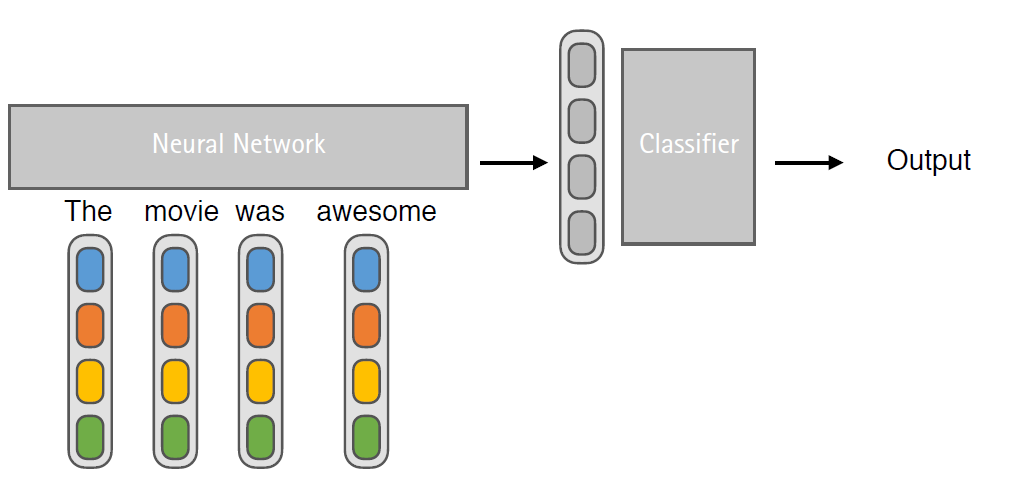
\includegraphics[scale=.4]{bild17}
    \end{figure}
\end{frame}


\begin{frame}{Saliency Maps for Language}
    \begin{itemize}
        \item We obtain gradients per dimension but we want attributions or importance scores at
the level of world
        \item \textbf{Idea:} Simple aggregations of dimension-level gradients like sum, average, etc.
    \end{itemize}
    \begin{figure}
        \centering
        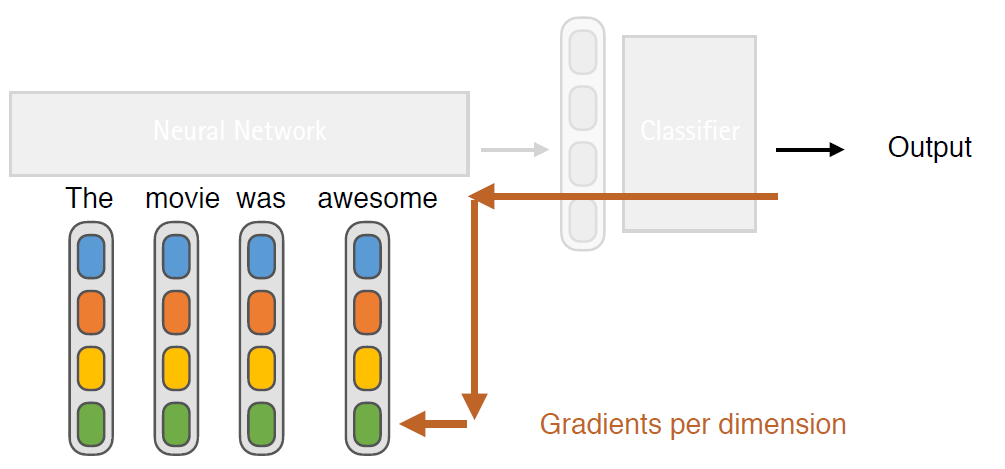
\includegraphics[scale=.4]{bild18}
    \end{figure}
\end{frame}

\begin{frame}{Saliency Maps - Setting}
    \begin{figure}
        \centering
        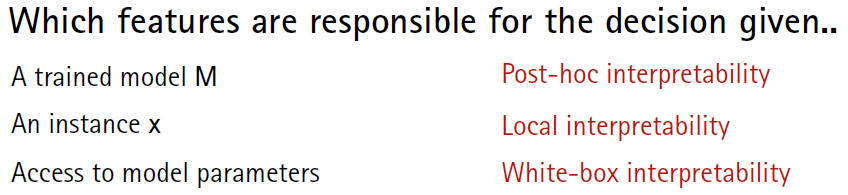
\includegraphics[width=0.6\linewidth]{bild19}
        \pause
        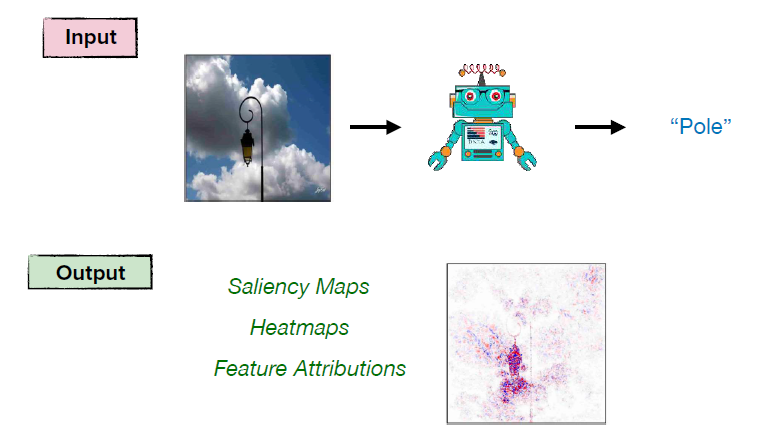
\includegraphics[width=0.6\linewidth]{bild20}
    \end{figure}
\end{frame}

\begin{frame}{Saliency Maps - Setting}
    \begin{figure}
        \centering
        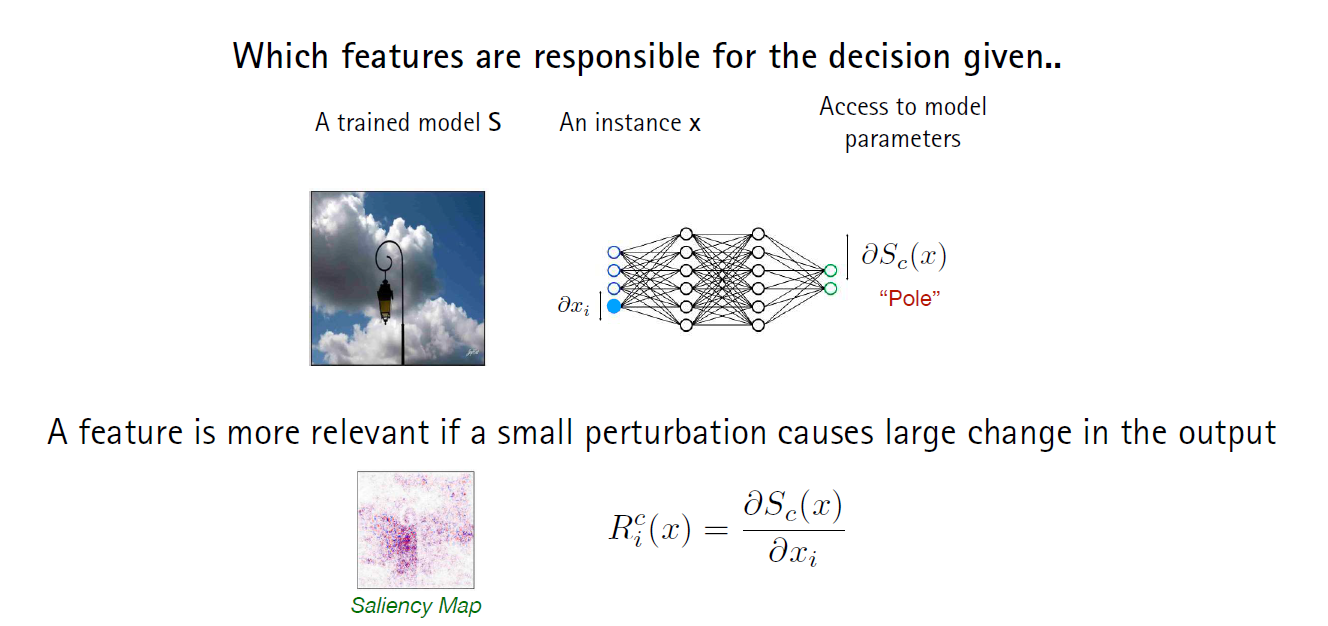
\includegraphics[scale=.4]{bild21}
    \end{figure}
\end{frame}

\begin{frame}{Problems with Deep Nets}

    \begin{figure}
        \centering
        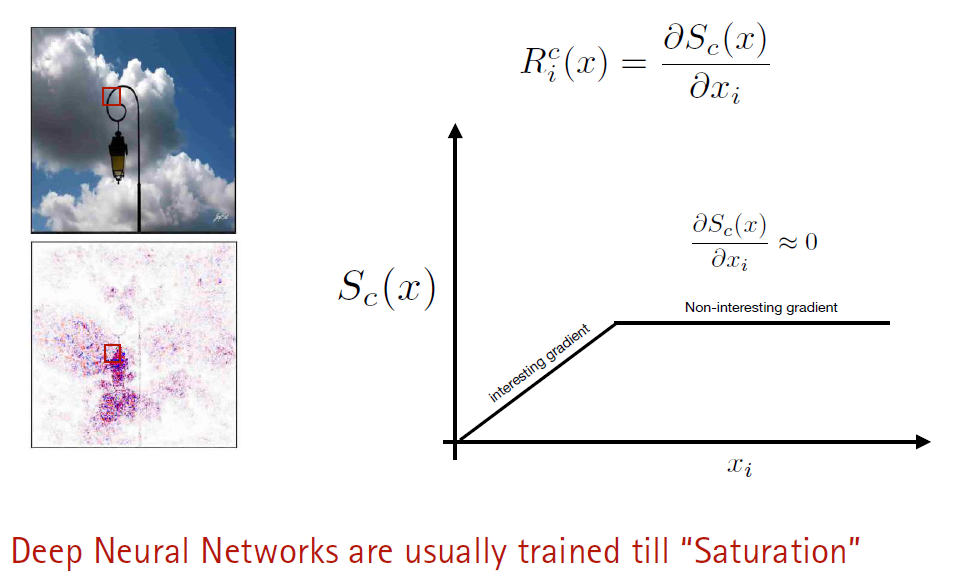
\includegraphics[width=0.6\linewidth]{bild22}
    \end{figure}
\end{frame}

\begin{frame}{Perturbing Inputs}
\begin{itemize}
    \item Small perturbations at the saturation point do not give us interesting gradients
    \item Extreme perturbation (to say a baseline image) can give us interesting gradients
\end{itemize}
\begin{figure}
    \centering
    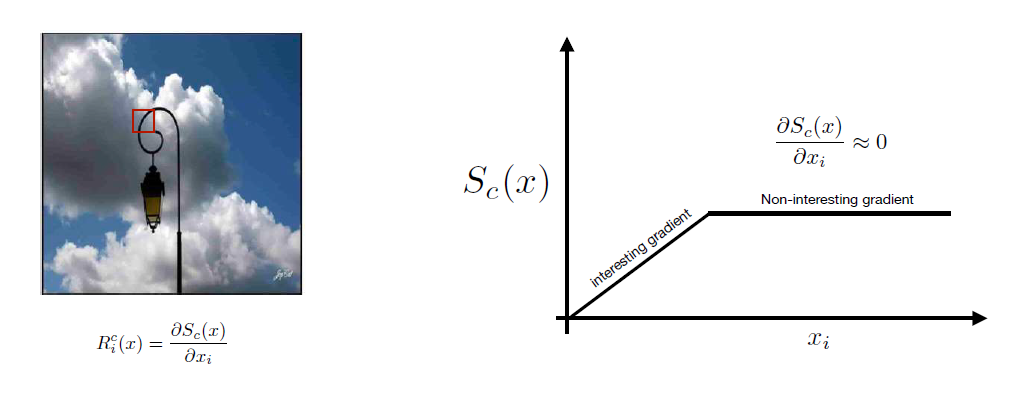
\includegraphics[scale=.5]{bild23}
\end{figure}
\end{frame}

\begin{frame}{Integrated Gradients}
    Compute gradient estimate based on gradients over a path of specific perturbations
    \begin{figure}
    \bigskip
    \bigskip
       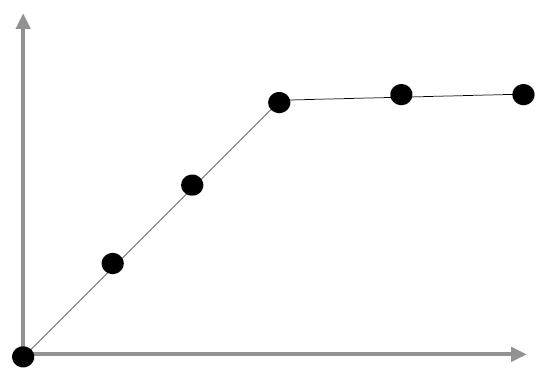
\includegraphics[width=0.6\linewidth]{bild28}
    \end{figure}
\end{frame}

\begin{frame}{Integrated Gradients}
    Compute gradient estimate based on gradients over a path of specific perturbations\\
    Choose a Baseline to contrast %
\includegraphics[width=0.1\linewidth]{black}
    \begin{figure}
    \bigskip
    \bigskip
       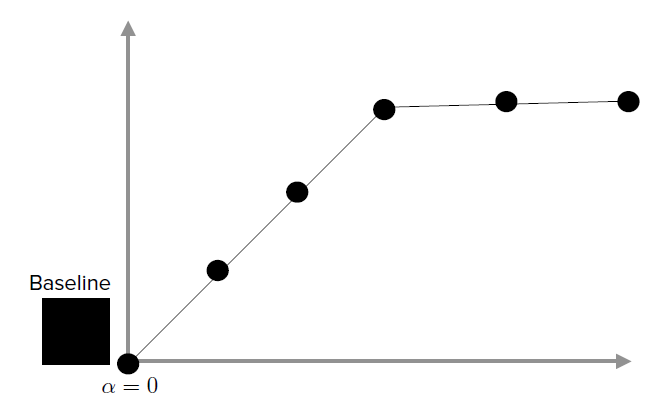
\includegraphics[width=0.6\linewidth]{bild29}
    \end{figure}
\end{frame}

\begin{frame}{Integrated Gradients}
    Compute gradient estimate based on gradients over a path of specific perturbations\\
    Choose a Baseline to contrast %
\includegraphics[scale=.3]{black}
    \begin{figure}
    \bigskip
    \bigskip
       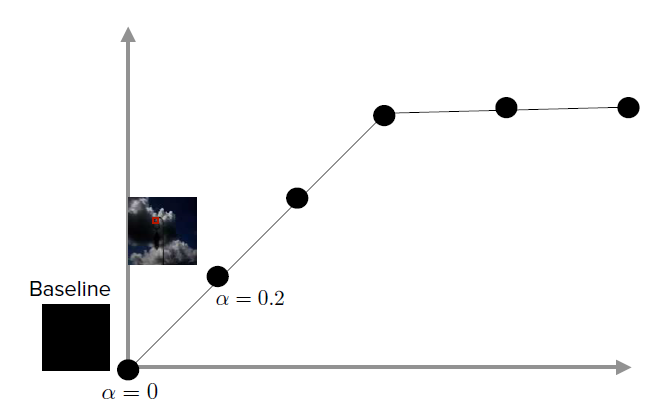
\includegraphics[width=0.6\linewidth]{bild30}
    \end{figure}
\end{frame}


\begin{frame}{Integrated Gradients}
    Compute gradient estimate based on gradients over a path of specific perturbations\\
    Choose a Baseline to contrast %
\includegraphics[scale=.3]{black}
    \begin{figure}
    \bigskip
    \bigskip
       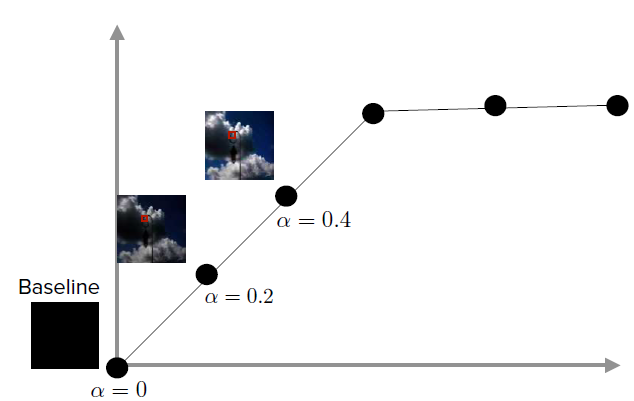
\includegraphics[width=0.6\linewidth]{bild31}
    \end{figure}
\end{frame}


\begin{frame}{Integrated Gradients}
    Compute gradient estimate based on gradients over a path of specific perturbations\\
    Choose a Baseline to contrast %
\includegraphics[scale=.3]{black}
    \begin{figure}
    \bigskip
    \bigskip
       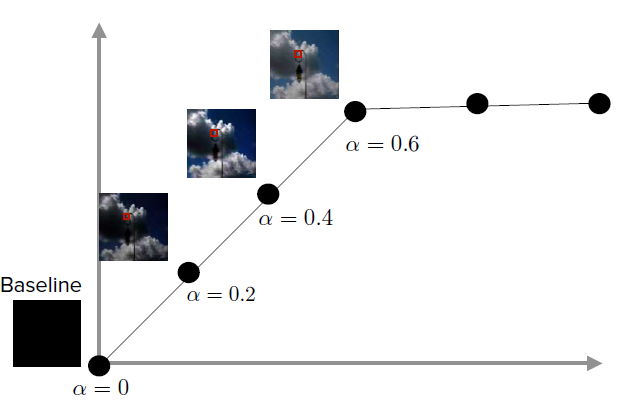
\includegraphics[width=0.6\linewidth]{bild32}
    \end{figure}
\end{frame}

\begin{frame}{Integrated Gradients}
    Compute gradient estimate based on gradients over a path of specific perturbations\\
    Choose a Baseline to contrast %
\includegraphics[scale=.3]{black}
    \begin{figure}
    \bigskip
    \bigskip
       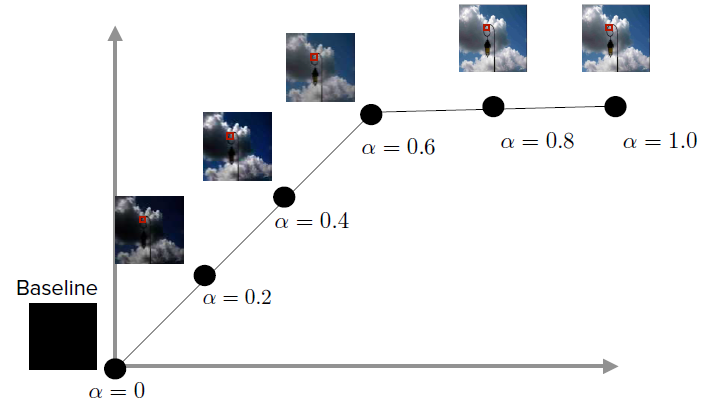
\includegraphics[width=0.6\linewidth]{bild33}
    \end{figure}
\end{frame}

\begin{frame}{Integrated Gradients}
\begin{enumerate}
    \item Choose a Baseline to contrast
    \item Compute gradients at different mask values
    \item Attribution = Aggregation over gradients computed for a certain set of perturbations
\end{enumerate}
\bigskip

\begin{equation*}
   R^c_i(x) = x_i \cdot \int^1_{\alpha = 0} \frac{\partial S_c(\Tilde{x})}{\partial(\Tilde{x}_i)}d\alpha
\end{equation*}

where $\Tilde{x}=\overline{x}+\alpha(x-\overline{x})$


$$
$$

Integrated Gradients monitors how the network changes from a zero signal input to actual
input through the use of gradients
\end{frame}

\begin{frame}{Baseline}
    \begin{itemize}
        \item Baseline is an information less input
        \item The choice of baselines matters a lot and is typically domain dependent
        \begin{itemize}
            \item Black or gray images
            \item Zero embedding in language
            \item Random document in retrieval
        \end{itemize}
    \end{itemize}
    \begin{figure}
        \centering
        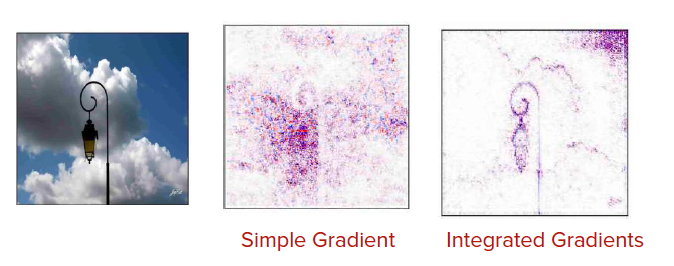
\includegraphics[scale=.5]{bild25}
    \end{figure}
\end{frame}

\begin{frame}{SmoothGrad}
    \begin{itemize}
        \item Gradients are local ways to measure sensitivity
        \item In highly nonlinear loss surfaces you obtain quite noisy gradients
        \begin{itemize}
            \item In this figure, majority of the neighbourhood gives positive gradient
        \end{itemize}
    \end{itemize}
    \begin{figure}
        \centering
        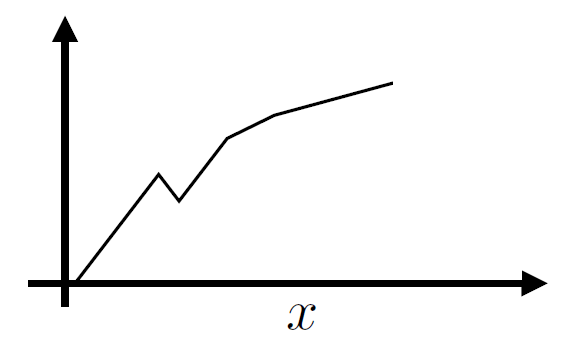
\includegraphics[width=0.6\linewidth]{bild26}
    \end{figure}
\end{frame}

\begin{frame}{SmoothGrad}
    \begin{itemize}
        \item Calculate multiple copies of the input with a small noise (usually Gaussian noise)
        \item Actual gradient is the average of the gradients of each of the copies
    \end{itemize}
    \begin{figure}
        \centering
        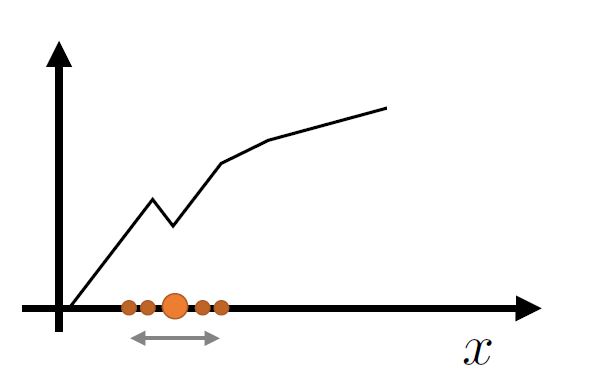
\includegraphics[width=0.6\linewidth]{bild27}
    \end{figure}
\end{frame}

\begin{frame}{Conclusion}
\begin{itemize}
    \item Gradients are central in computing feature attributions and are visualised using
saliency maps
\item Simple gradient-based approaches for neural networks attribute the importance back to
the input features
\item Deep learning models suffer from critical problems for gradient-based methods
\begin{itemize}
    \item Models are trained to saturation given near-zero gradients — Integrated Gradients
    \item Gradients are unstable due to highly non-linear loss surface — SmoothGrad
\end{itemize}
\item Tons of other approaches proposed in the literature
\item Caution that explanations might disagree with each other
\item Caution that gradient-based approaches need to be adapted depending on the input
style
\end{itemize}
\end{frame}

\endlecture
\end{document}